% ====================================================================================
\chapter{神经算子：从函数到函数的映射}
% ====================================================================================

% ====================================================================================
\section*{引言：一次训练，任意条件}
% ====================================================================================

\sidenoteplain{神经算子的两个里程碑工作几乎同时出现：Lu Lu等人在2019年提出DeepONet，Zongyi Li等人在2020年提出FNO。两种方法代表了不同的设计哲学——DeepONet基于万能逼近定理，FNO利用傅里叶变换的效率。}

\storynote{Lu Lu}{Karniadakis 的学生，DeepONet 第一作者，也是开源库 DeepXDE 的作者——PINN 与神经算子研究的事实标准工具。DeepONet 的理论基础是 Tianping Chen 与 Hong Chen 1995 年的算子万能逼近定理，一个被埋没了二十多年的结果。}

在上一章中，我们学习了PINN：用神经网络逼近一个特定PDE的解。但你可能已经意识到一个问题：

\begin{quote}
\textit{每次初始条件或边界条件变化，我们都要重新训练网络。这太低效了！}
\end{quote}

想象一下天气预报的场景：大气动力学方程是固定的（Navier-Stokes方程），但每天的初始状态都不同。如果用PINN，每天凌晨都要花几个小时重新训练网络——这显然不切实际。

有没有办法\textbf{一次训练，对任意初始条件都能直接预测}？

这就是\textbf{神经算子}（Neural Operator）的目标：不是学习一个特定的解函数$u(x)$，而是学习从"条件函数"到"解函数"的\textbf{映射}。

\vspace{0.3cm}
\noindent\textit{为什么天气预报模型可以"一次训练、天天用"，而 PINN 却要天天重训？为什么一个在 64 个格点上训练的网络，可以直接在 256 个格点上推理？第6章辛辛苦苦组装的刚度矩阵 $K$，和这里学出来的"算子"是什么关系？}

\begin{quote}
\textbf{本章目标}：让你看到神经算子不是又一个新架构，而是第6章那句"解方程就是算 $K^{-1}F$"的直接延伸：第6章我们辛辛苦苦组装 $K$ 再去解，本章干脆从数据里把 $K^{-1}$——也就是格林函数——学出来。读完本章你会明白，为什么"一次训练、任意条件"是可能的，为什么它与网格分辨率无关，以及当我们把约束（物理定律）从损失函数里拿掉时，究竟丢掉了什么。
\end{quote}

\begin{tcolorbox}[colback=green!5, colframe=green!60!black, title=学完这章，你将能够...]
\begin{itemize}
    \item 解释为什么神经算子比PINN更适合实时预测
    \item 实现一个简化版DeepONet学习一个简单算子（反导数算子；热传导方程见习题）
    \item 理解FNO如何用傅里叶变换实现高效的全局卷积
    \item 分析神经算子与格林函数的数学联系
    \item 评估神经算子在给定任务上的适用性
\end{itemize}
\end{tcolorbox}

% ====================================================================================
\section{从求解到映射：算子学习的思想}
% ====================================================================================

\subsection{PINN的局限性}

回顾PINN的工作方式：

\begin{center}
\begin{tikzpicture}[
    box/.style={rectangle, draw, minimum width=2.5cm, minimum height=1cm, align=center},
    arrow/.style={-{Stealth}, thick}
]
    \node[box] (input) at (0, 0) {初始条件\\$u_0(x)$};
    \node[box] (pinn) at (4, 0) {PINN\\训练};
    \node[box] (output) at (8, 0) {解\\$u(x,t)$};
    
    \draw[arrow] (input) -- (pinn);
    \draw[arrow] (pinn) -- (output);
    
    \node[below=0.5cm of pinn, text=red] {每次新条件都要重训！};
\end{tikzpicture}
\end{center}

具体地，考虑热传导方程：
\begin{equation}
    \frac{\partial u}{\partial t} = \alpha \frac{\partial^2 u}{\partial x^2}, \quad u(x, 0) = u_0(x)
\end{equation}

如果$u_0(x) = \sin(\pi x)$，我们训练一个PINN得到解$u_1(x,t)$。

现在换一个初始条件$u_0(x) = \sin(2\pi x)$，我们必须\textbf{从头训练}另一个PINN得到$u_2(x,t)$。

\begin{example}[PINN的计算成本]
假设：
\begin{itemize}
    \item 训练一个PINN需要10分钟
    \item 我们需要预测1000个不同初始条件下的解
\end{itemize}
那么总计算时间是$10 \times 1000 = 10000$分钟 $\approx$ 7天！

这对于需要实时预测的应用（如天气预报）是完全不可接受的。
\end{example}

\subsection{算子学习的目标}

算子学习的思路是：既然方程是固定的，不同的只是初始/边界条件，那么我们应该学习的是\textbf{从条件到解的映射}。

\begin{definition}[解算子]
考虑PDE：
\begin{equation}
    \mathcal{L}[u] = f, \quad u|_{\partial\Omega} = g, \quad u|_{t=0} = u_0
\end{equation}
\textbf{解算子}$\mathcal{G}$是从初始/边界条件到解的映射：
\begin{equation}
    \mathcal{G}: u_0 \mapsto u
\end{equation}
其中$u_0$是输入函数，$u$是输出函数。
\end{definition}
\review{第6章}{有限元把 $-\nabla^2 u = f$ 变成 $KU = F$，解是 $U = K^{-1}F$。$K$ 只依赖方程和网格，不依赖载荷：换一个 $F$ 只需再乘一次 $K^{-1}$。"解算子"就是 $K^{-1}$ 的连续版本——本章要学的正是它。}

\begin{center}
\begin{tikzpicture}[
    box/.style={rectangle, draw, minimum width=2.5cm, minimum height=1cm, align=center},
    arrow/.style={-{Stealth}, thick}
]
    \node[box] (input1) at (0, 1) {$u_0^{(1)}(x)$};
    \node[box] (input2) at (0, 0) {$u_0^{(2)}(x)$};
    \node[box] (input3) at (0, -1) {$u_0^{(3)}(x)$};
    
    \node[box, minimum height=3cm] (operator) at (4, 0) {神经算子\\$\mathcal{G}_\theta$\\（一次训练）};
    
    \node[box] (output1) at (8, 1) {$u^{(1)}(x,t)$};
    \node[box] (output2) at (8, 0) {$u^{(2)}(x,t)$};
    \node[box] (output3) at (8, -1) {$u^{(3)}(x,t)$};
    
    \draw[arrow] (input1) -- (operator);
    \draw[arrow] (input2) -- (operator);
    \draw[arrow] (input3) -- (operator);
    \draw[arrow] (operator) -- (output1);
    \draw[arrow] (operator) -- (output2);
    \draw[arrow] (operator) -- (output3);
    
    \node[below=0.5cm of operator, text=blue] {训练后，任意新条件直接推理！};
\end{tikzpicture}
\end{center}

\begin{insightbox}
\textbf{传统神经网络} vs \textbf{神经算子}：

\begin{center}
\begin{tabular}{l|cc}
\toprule
& \textbf{传统神经网络} & \textbf{神经算子} \\
\midrule
输入 & 向量 $x \in \mathbb{R}^n$ & 函数 $u(x)$ \\
输出 & 向量 $y \in \mathbb{R}^m$ & 函数 $v(x)$ \\
学习目标 & $f: \mathbb{R}^n \to \mathbb{R}^m$ & $\mathcal{G}: \mathcal{U} \to \mathcal{V}$ \\
\bottomrule
\end{tabular}
\end{center}

神经算子是\textbf{函数空间到函数空间}的映射！
\end{insightbox}

\subsection{为什么这很难？}

函数是无穷维对象，如何用有限参数的神经网络来表示"函数到函数"的映射？

传统方法是离散化：把函数$u(x)$在网格点$\{x_1, \ldots, x_n\}$上采样，得到向量$(u(x_1), \ldots, u(x_n))$，然后用传统神经网络处理。

但这有几个问题：
\begin{enumerate}
    \item \textbf{分辨率绑定}：在$32 \times 32$网格上训练的网络，不能直接用于$64 \times 64$的输入
    \item \textbf{缺乏泛化性}：网络学到的是"像素到像素"的映射，而不是"函数到函数"的映射
    \item \textbf{网格依赖}：换一种网格划分方式，就需要重新训练
\end{enumerate}

神经算子的核心挑战是：如何设计一个\textbf{与离散化方式无关}的架构？

% ====================================================================================
\section{离散化无关性：神经算子的核心特性}
% ====================================================================================

\subsection{什么是离散化无关性}

\begin{definition}[离散化无关性]
一个神经算子$\mathcal{G}_\theta$具有\textbf{离散化无关性}（discretization invariance），如果：
\begin{enumerate}
    \item 它可以接受任意分辨率的输入
    \item 它可以在任意分辨率上输出
    \item 无论使用什么分辨率，它都在逼近同一个连续算子
\end{enumerate}
\end{definition}

用数学语言说：设$\mathcal{G}^*$是真实的连续算子，$\mathcal{G}_\theta^{(n)}$是在$n$个网格点上的离散近似。离散化无关性意味着：
\begin{equation}
    \lim_{n \to \infty} \mathcal{G}_\theta^{(n)} = \mathcal{G}_\theta \quad \text{（在适当范数意义下）}
\end{equation}
\clarify{离散化无关性保证的是：分辨率 $n \to \infty$ 时 $\mathcal{G}_\theta^{(n)}$ 收敛到某个与网格无关的连续算子 $\mathcal{G}_\theta$。它是否等于真实的 $\mathcal{G}^*$，取决于训练得好不好——那是另一回事。}

\begin{example}[零样本超分辨率]
这是离散化无关性最惊人的应用：

假设我们在$32 \times 32$的粗网格上训练了一个FNO模型。训练完成后，我们可以：
\begin{itemize}
    \item 输入$64 \times 64$的数据，得到$64 \times 64$的输出
    \item 输入$128 \times 128$的数据，得到$128 \times 128$的输出
    \item 输入$256 \times 256$的数据，得到$256 \times 256$的输出
\end{itemize}
\textbf{无需任何额外训练！}

这被称为\textbf{零样本超分辨率}（zero-shot super-resolution）。
\end{example}

\subsection{为什么传统CNN不具有离散化无关性？}

考虑一个简单的1D卷积：
\begin{equation}
    (k * u)_i = \sum_{j=-r}^{r} k_j \cdot u_{i+j}
\end{equation}

这里$k$是一个固定大小的卷积核（如$3 \times 3$）。问题在于：

\begin{itemize}
    \item 卷积核大小是固定的像素数，而不是固定的物理尺寸
    \item 在不同分辨率下，同样大小的卷积核覆盖的物理区域不同
\end{itemize}

\begin{example}[卷积核的分辨率依赖]
假设物理域是$[0, 1]$，使用$3 \times 3$卷积核：
\begin{itemize}
    \item 在$32$个网格点上：卷积核覆盖物理尺寸$3 \times \frac{1}{32} \approx 0.094$
    \item 在$64$个网格点上：卷积核覆盖物理尺寸$3 \times \frac{1}{64} \approx 0.047$
\end{itemize}

同样的卷积核，在不同分辨率下"看到"的物理区域完全不同！
\end{example}

\subsection{如何实现离散化无关性？}

有两种主要思路：

\textbf{思路1：在函数空间定义操作}

不要在"像素"上定义操作，而是在"函数"上定义操作。具体方法是使用\textbf{积分算子}：
\begin{equation}
    (Ku)(x) = \int_\Omega \kappa(x, y) u(y) \, dy
\end{equation}

积分是定义在连续函数上的，与离散化方式无关。不同分辨率只是对同一个积分的不同数值近似。

\textbf{思路2：在频域操作}

傅里叶变换将函数映射到频域。频域表示是"坐标无关"的——频率$k$的傅里叶系数对应的是函数的全局特性，与网格划分无关。

% ====================================================================================
\section{数学统一：格林函数与积分变换}
% ====================================================================================

在深入具体架构之前，让我们建立一个统一的数学框架。

\begin{tcolorbox}[colback=yellow!10, colframe=orange!80, title=本章的核心观点]
\textbf{本章的问题仍是第1章的拉格朗日乘子法，只是这次我们不求某一个问题的解，而是求"约束放松一点、解变多少"这张影子价格表本身。}

线性情形下这张表有名字：格林函数 $G(x, \xi) = \partial u(x)/\partial f(\xi)$，也就是第6章 $K^{-1}$ 的连续版本。神经算子把它推广到非线性方程，并直接从数据里学。

\begin{center}
\renewcommand{\arraystretch}{1.3}
\small
\begin{tabular}{lll}
\toprule
 & \textbf{第1章 / 第6章} & \textbf{本章（神经算子）} \\
\midrule
变量 & $x \in \R^n$ / 节点值 $U$ & 算子参数 $\theta$（一次学完一族问题） \\
目标 & $f(x)$ / $\frac{1}{2}U^\top KU - F^\top U$ & 数据误差 $\sum_i \|\mathcal{G}_\theta(a_i) - u_i\|^2$ \\
约束 & $g(x) = 0$ / 无（已在能量里） & 纯数据驱动：无显式约束；PINO：$\mathcal{N}[\mathcal{G}_\theta(a)] = f$ \\
乘子 & $\lambda$（影子价格） & 格林函数 $G(x, \xi) = \partial u(x)/\partial f(\xi)$：对源项的影子价格表 \\
一阶条件 & $\nabla f + \lambda^\top \nabla g = 0$ / $KU = F$ & $u = \int G(x, \xi) f(\xi)\,d\xi$，即 $U = K^{-1}F$ \\
求解方式 & 组装 $K$，解方程 & 跳过组装，直接学 $K^{-1}$（$\kappa_\theta$、$R(k)$、$b_k t_k$） \\
\bottomrule
\end{tabular}
\end{center}
\end{tcolorbox}

\subsection{线性PDE的解算子}

考虑线性PDE：
\begin{equation}
    \mathcal{L}[u] = f
\end{equation}
其中$\mathcal{L}$是线性微分算子（如$-\nabla^2$）。

\begin{theorem}[格林函数表示]
\label{thm:green}
如果格林函数$G(x, y)$满足：
\begin{equation}
    \mathcal{L}_x[G(x, y)] = \delta(x - y)
\end{equation}
且 $G(\cdot, y)$ 满足齐次边界条件，那么PDE的解可以写成积分形式：
\begin{equation}
    u(x) = \int_\Omega G(x, y) f(y) \, dy
\end{equation}
\end{theorem}

\begin{proof}
将$u(x) = \int G(x, y) f(y) dy$代入方程：
\begin{align}
    \mathcal{L}[u](x) &= \mathcal{L}_x\left[\int_\Omega G(x, y) f(y) \, dy\right] \\
    &= \int_\Omega \mathcal{L}_x[G(x, y)] f(y) \, dy \quad \text{（线性性）} \\
    &= \int_\Omega \delta(x - y) f(y) \, dy \\
    &= f(x) \quad \checkmark
\end{align}
（边界条件由 $G(\cdot, y)$ 满足齐次边界条件保证。）
\end{proof}
\review{第1章}{影子价格 $\lambda = -df^*/d\epsilon$：约束放松一点，最优值变多少。现在的约束是"每个点 $\xi$ 处方程都成立"，无穷多条；在 $\xi$ 处放松一个单位源 $\delta(x - \xi)$，解在 $x$ 处变化 $G(x, \xi)$。格林函数就是一整张影子价格表，第9章的伴随变量就是这张表乘上目标的梯度。}

\begin{example}[一维泊松方程的格林函数]
考虑：
\begin{equation}
    -u''(x) = f(x), \quad x \in (0, 1), \quad u(0) = u(1) = 0
\end{equation}

格林函数为：
\begin{equation}
    G(x, y) = \begin{cases}
        y(1-x), & y < x \\
        x(1-y), & y \geq x
    \end{cases}
\end{equation}

解为：
\begin{equation}
    u(x) = \int_0^1 G(x, y) f(y) \, dy
\end{equation}
\end{example}

回想第6章：有限元把这个方程变成 $KU = F$，解是 $U = K^{-1}F$。刚度矩阵 $K$ 只和方程、网格有关，与载荷无关——换一个 $F$，只需再乘一次 $K^{-1}$。所以"解算子"就是 $K^{-1}$，格林函数 $G(x, y)$ 就是 $K^{-1}$ 的连续版本：对一维泊松方程，$K^{-1}$ 的第 $(i, j)$ 元恰好等于 $h\, G(x_i, x_j)$。第6章我们组装 $K$ 再解方程；本章跳过组装，直接从数据里学 $K^{-1}$。
\tryit{用第6章的代码组装一维泊松方程的刚度矩阵 $K = \frac{1}{h}\,\mathrm{tridiag}(-1, 2, -1)$（$h = 0.1$），算 $K^{-1}$ 并画热力图，与 $G(x, y) = \min(x, y)(1 - \max(x, y))$ 对比：$K^{-1}$ 的第 $(i, j)$ 元恰好等于 $h\, G(x_i, x_j)$。}

\subsection{神经算子的统一形式}

定理\ref{thm:green}告诉我们：线性PDE的解算子本质上是一个\textbf{积分算子}。

这启发了神经算子的设计：

\begin{keyformula}[title=神经算子的核心形式]
所有神经算子都可以写成积分变换的形式：
\begin{equation}
    v(x) = \sigma\left( Wu(x) + \int_\Omega \kappa_\theta(x, y) u(y) \, dy + b(x) \right)
\end{equation}
其中：
\begin{itemize}
    \item $\kappa_\theta(x, y)$是\textbf{可学习的积分核}（类比格林函数）
    \item $W$是局部线性变换
    \item $\sigma$是非线性激活函数
    \item $b(x)$是偏置
\end{itemize}
\end{keyformula}

\begin{unification}[title=不同神经算子架构的统一]
不同的神经算子架构，本质上是选择了不同的方式来参数化积分核$\kappa_\theta(x, y)$：

\begin{center}
\begin{tabular}{l|l}
\toprule
\textbf{架构} & \textbf{积分核的形式} \\
\midrule
DeepONet & $\sum_k b_k(u)\, t_k(x)$：分支给系数、主干给基函数（分支为线性层时 $\kappa(x,y) = \sum_k t_k(x) \sum_j w_{kj}\delta(y - y_j)$；一般情形对 $u$ 非线性，已超出线性积分算子族） \\
FNO & $\kappa(x, y) = \kappa(x - y)$（平移不变，频域表示） \\
GNO & 图上的消息传递（非规则网格） \\
Transformer & $\kappa(x, y) = \text{softmax}(Q(x)K(y)^T / \sqrt{d})$（数据依赖） \\
\bottomrule
\end{tabular}
\end{center}
\end{unification}
\think{分支网络 $b_k(u)$ 对 $u$ 是非线性的，所以 DeepONet 写不成对 $u$ 线性的 $\int \kappa(x, y) u(y)\,dy$。那它和积分算子框架"统一"在哪里？提示：把分支网络换成线性层，看看 $\kappa$ 长什么样。}

% ====================================================================================
\section{DeepONet：基函数展开视角}
\label{sec:deeponet}
% ====================================================================================

\subsection{万能逼近定理}

DeepONet的理论基础是Chen \& Chen在1995年证明的万能逼近定理：

\begin{theorem}[算子的万能逼近定理]
设$\mathcal{G}: \mathcal{U} \to \mathcal{V}$是从紧集$K \subset C(\Omega_1)$到$C(\Omega_2)$的非线性连续算子。那么对于任意$\epsilon > 0$，存在正整数$p$、连续函数$g_k$、$f_k$和点$\{y_j\}_{j=1}^m \subset \Omega_1$，使得：
\begin{equation}
    \left| \mathcal{G}(u)(x) - \sum_{k=1}^{p} \underbrace{g_k\left(u(y_1), \ldots, u(y_m)\right)}_{\text{依赖于输入函数}} \cdot \underbrace{f_k(x)}_{\text{依赖于输出位置}} \right| < \epsilon
\end{equation}
对所有$u \in K$和$x \in \Omega_2$成立。
\end{theorem}

\begin{remark}[直觉理解]
这个定理说的是：任何算子都可以近似为"\textbf{系数}"乘以"\textbf{基函数}"的形式，其中：
\begin{itemize}
    \item 系数$g_k(u(y_1), \ldots, u(y_m))$依赖于输入函数在某些"传感器"位置的值
    \item 基函数$f_k(x)$只依赖于输出位置
\end{itemize}

这类似于傅里叶级数$f(x) = \sum_k c_k e^{ikx}$，只是这里的"傅里叶系数"$c_k$变成了输入函数的非线性泛函。
\end{remark}

\subsection{DeepONet架构}

基于万能逼近定理，DeepONet设计了一个"双塔"结构：

\begin{definition}[DeepONet]
DeepONet由两个子网络组成：
\begin{itemize}
    \item \textbf{分支网络}（Branch Net）$\mathbf{b}_\theta$：输入为函数$u$在传感器位置的采样值$(u(y_1), \ldots, u(y_m))$，输出为$p$维向量$(b_1, \ldots, b_p)$
    \item \textbf{主干网络}（Trunk Net）$\mathbf{t}_\phi$：输入为查询位置$x$，输出为$p$维向量$(t_1, \ldots, t_p)$
\end{itemize}

最终输出通过内积计算：
\begin{equation}
    \mathcal{G}_{\theta, \phi}(u)(x) = \sum_{k=1}^{p} b_k(u) \cdot t_k(x) = \mathbf{b}_\theta(u) \cdot \mathbf{t}_\phi(x)
\end{equation}
\end{definition}
\review{第6章}{$\sum_k b_k(u)\, t_k(x)$ 和有限元的 $u_h(x) = \sum_j U_j \phi_j(x)$ 是同一种写法：主干网络学"基函数" $\phi_j$，分支网络学"系数" $U_j$ 对载荷的依赖，也就是 $K^{-1}F$ 这一步。区别只是基函数不再是固定的帐篷函数，而是学出来的。}

\begin{figure}[htbp]
\centering
\begin{tikzpicture}[
    box/.style={rectangle, draw, rounded corners, minimum width=2cm, minimum height=0.8cm, align=center},
    arrow/.style={-{Stealth}, thick}
]
    % Branch Net
    \node[box, fill=blue!20] (sensors) at (0, 2) {传感器值\\$(u(y_1), \ldots, u(y_m))$};
    \node[box, fill=blue!30] (branch) at (0, 0) {分支网络\\(MLP)};
    \node[box, fill=blue!10] (b) at (0, -2) {$\mathbf{b} = (b_1, \ldots, b_p)$};
    
    % Trunk Net
    \node[box, fill=green!20] (query) at (6, 2) {查询位置\\$x$};
    \node[box, fill=green!30] (trunk) at (6, 0) {主干网络\\(MLP)};
    \node[box, fill=green!10] (t) at (6, -2) {$\mathbf{t} = (t_1, \ldots, t_p)$};
    
    % Output
    \node[box, fill=red!20] (output) at (3, -4) {$\mathcal{G}(u)(x) = \mathbf{b} \cdot \mathbf{t}$};
    
    % Arrows
    \draw[arrow] (sensors) -- (branch);
    \draw[arrow] (branch) -- (b);
    \draw[arrow] (query) -- (trunk);
    \draw[arrow] (trunk) -- (t);
    \draw[arrow] (b) -- (output);
    \draw[arrow] (t) -- (output);
\end{tikzpicture}
\caption{DeepONet的双塔架构}
\label{fig:deeponet}
\end{figure}

\subsection{物理直觉：POD分解}

DeepONet的形式让人联想到\textbf{本征正交分解}（Proper Orthogonal Decomposition，POD）。

在POD中，我们将参数化的解$u(x; \mu)$分解为：
\begin{equation}
    u(x; \mu) \approx \sum_{k=1}^{p} \alpha_k(\mu) \phi_k(x)
\end{equation}
其中$\{\phi_k\}$是数据驱动的基函数，$\alpha_k(\mu)$是依赖于参数的系数。

DeepONet可以看作是POD的\textbf{神经网络版本}：
\begin{itemize}
    \item 主干网络学习"基函数"$t_k(x)$
    \item 分支网络学习"系数"$b_k(u)$对输入函数的依赖
\end{itemize}

\begin{remark}[为什么用内积？]
内积$\mathbf{b} \cdot \mathbf{t}$是一种"双线性"操作：
\begin{itemize}
    \item 固定$u$，输出是$x$的非线性函数（通过主干网络）
    \item 固定$x$，输出是$u$的非线性函数（通过分支网络）
\end{itemize}

这种结构允许两个网络独立地编码各自的信息，然后通过简单的内积组合。也可以用其他组合方式（如拼接后过MLP），但内积最简洁高效。
\end{remark}

\subsection{完整代码实现}

\begin{lstlisting}[language=Python, caption={DeepONet的完整实现}]
import torch
import torch.nn as nn
import numpy as np

class DeepONet(nn.Module):
    """
    DeepONet: 学习函数到函数的映射
    
    架构：
    - 分支网络：编码输入函数 u 在传感器位置的值
    - 主干网络：编码输出查询位置 x
    - 输出：两个网络输出的内积
    """
    
    def __init__(self, 
                 n_sensors,      # 传感器数量（输入函数的采样点数）
                 branch_layers,  # 分支网络层结构，如 [100, 64, 64, 64]
                 trunk_layers,   # 主干网络层结构，如 [1, 64, 64, 64]
                 p):             # 输出维度（"基函数"数量）
        super().__init__()
        
        # ========== 分支网络 ==========
        # 输入：u在传感器位置的值，形状 (batch, n_sensors)
        # 输出：系数向量，形状 (batch, p)
        branch_layers = [n_sensors] + branch_layers + [p]
        self.branch_net = self._build_mlp(branch_layers)
        
        # ========== 主干网络 ==========
        # 输入：查询位置 x，形状 (batch, input_dim)
        # 输出：基函数值，形状 (batch, p)
        trunk_layers = trunk_layers + [p]
        self.trunk_net = self._build_mlp(trunk_layers)
        
        # 偏置项
        self.bias = nn.Parameter(torch.zeros(1))
        
    def _build_mlp(self, layers):
        """构建MLP"""
        net = []
        for i in range(len(layers) - 1):
            net.append(nn.Linear(layers[i], layers[i+1]))
            if i < len(layers) - 2:  # 最后一层不加激活
                net.append(nn.Tanh())
        return nn.Sequential(*net)
    
    def forward(self, u_sensors, x_query):
        """
        前向传播
        
        参数:
            u_sensors: 输入函数在传感器的值, 形状 (batch, n_sensors)
            x_query: 查询位置, 形状 (batch, input_dim) 或 (batch, n_query, input_dim)
        
        返回:
            G(u)(x): 算子输出, 形状与x_query对应
        """
        # 分支网络：编码输入函数
        b = self.branch_net(u_sensors)  # (batch, p)
        
        # 主干网络：编码查询位置
        # 处理不同形状的x_query
        if x_query.dim() == 2:
            t = self.trunk_net(x_query)  # (batch, p)
            # 内积
            output = torch.sum(b * t, dim=-1, keepdim=True) + self.bias
        else:
            # x_query: (batch, n_query, input_dim)
            batch_size, n_query, input_dim = x_query.shape
            x_flat = x_query.reshape(-1, input_dim)  # (batch*n_query, input_dim)
            t_flat = self.trunk_net(x_flat)  # (batch*n_query, p)
            t = t_flat.reshape(batch_size, n_query, -1)  # (batch, n_query, p)
            
            # b: (batch, p) -> (batch, 1, p)
            b = b.unsqueeze(1)
            # 内积: (batch, n_query)
            output = torch.sum(b * t, dim=-1) + self.bias
        
        return output


def demo_deeponet_antiderivative():
    """
    演示：用DeepONet学习反导数算子
    
    目标算子：G(u)(x) = integral_0^x u(t) dt
    """
    torch.manual_seed(42)
    
    # ========== 参数设置 ==========
    n_sensors = 50      # 传感器数量
    n_train = 1000      # 训练样本数
    n_test = 100        # 测试样本数
    
    # ========== 生成数据 ==========
    def generate_data(n_samples, n_sensors, n_query=50):
        """
        生成训练数据
        
        输入函数：随机傅里叶级数
        u(x) = sum_k a_k * sin(k*pi*x) + b_k * cos(k*pi*x)
        
        输出：反导数 G(u)(x) = integral_0^x u(t) dt
        """
        x_sensors = torch.linspace(0, 1, n_sensors)
        x_query = torch.linspace(0, 1, n_query)
        
        U_sensors = []  # 输入函数在传感器的值
        X_query = []    # 查询位置
        Y_true = []     # 真实积分值
        
        for _ in range(n_samples):
            # 生成随机傅里叶系数
            n_modes = 5
            a = torch.randn(n_modes) * 0.5
            b = torch.randn(n_modes) * 0.5
            
            # 计算u(x) = sum_k a_k*sin(k*pi*x) + b_k*cos(k*pi*x)
            def u(x):
                result = torch.zeros_like(x)
                for k in range(1, n_modes + 1):
                    result += a[k-1] * torch.sin(k * np.pi * x)
                    result += b[k-1] * torch.cos(k * np.pi * x)
                return result
            
            # 计算积分的解析解
            # integral sin(k*pi*x) = -cos(k*pi*x)/(k*pi) + C
            # integral cos(k*pi*x) = sin(k*pi*x)/(k*pi) + C
            def integral_u(x):
                result = torch.zeros_like(x)
                for k in range(1, n_modes + 1):
                    # integral_0^x sin(k*pi*t) dt = (1 - cos(k*pi*x))/(k*pi)
                    result += a[k-1] * (1 - torch.cos(k * np.pi * x)) / (k * np.pi)
                    # integral_0^x cos(k*pi*t) dt = sin(k*pi*x)/(k*pi)
                    result += b[k-1] * torch.sin(k * np.pi * x) / (k * np.pi)
                return result
            
            U_sensors.append(u(x_sensors))
            X_query.append(x_query)
            Y_true.append(integral_u(x_query))
        
        U_sensors = torch.stack(U_sensors)  # (n_samples, n_sensors)
        X_query = torch.stack(X_query)      # (n_samples, n_query)
        Y_true = torch.stack(Y_true)        # (n_samples, n_query)
        
        return U_sensors, X_query.unsqueeze(-1), Y_true
    
    # 生成数据
    U_train, X_train, Y_train = generate_data(n_train, n_sensors)
    U_test, X_test, Y_test = generate_data(n_test, n_sensors)
    
    # ========== 创建模型 ==========
    model = DeepONet(
        n_sensors=n_sensors,
        branch_layers=[64, 64],
        trunk_layers=[1, 64, 64],
        p=64
    )
    
    optimizer = torch.optim.Adam(model.parameters(), lr=1e-3)
    
    # ========== 训练 ==========
    print("开始训练DeepONet...")
    n_epochs = 2000
    batch_size = 64
    
    for epoch in range(n_epochs):
        # 随机打乱
        perm = torch.randperm(n_train)
        total_loss = 0.0
        n_batches = 0
        
        for i in range(0, n_train, batch_size):
            idx = perm[i:i+batch_size]
            u_batch = U_train[idx]
            x_batch = X_train[idx]
            y_batch = Y_train[idx]
            
            # 前向传播
            y_pred = model(u_batch, x_batch)
            
            # 损失
            loss = torch.mean((y_pred - y_batch) ** 2)
            
            # 反向传播
            optimizer.zero_grad()
            loss.backward()
            optimizer.step()
            
            total_loss += loss.item()
            n_batches += 1
        
        if (epoch + 1) % 200 == 0:
            avg_loss = total_loss / n_batches
            print(f"Epoch {epoch+1}: MSE = {avg_loss:.6f}")
    
    # ========== 测试 ==========
    model.eval()
    with torch.no_grad():
        Y_pred = model(U_test, X_test)
        test_mse = torch.mean((Y_pred - Y_test) ** 2).item()
        print(f"\n测试集 MSE: {test_mse:.6f}")
        
        # 相对误差
        rel_error = torch.mean(torch.abs(Y_pred - Y_test) / (torch.abs(Y_test) + 1e-6))
        print(f"测试集相对误差: {rel_error:.4f}")
    
    print("\n训练完成！")

if __name__ == "__main__":
    demo_deeponet_antiderivative()
\end{lstlisting}

\begin{exercise}[title = 扩展DeepONet]
\begin{enumerate}
    \item 修改上述代码，让DeepONet学习\textbf{微分算子}$\mathcal{G}(u)(x) = u'(x)$。
    
    \textbf{提示}：微分比积分更难学（因为它是"不连续"的操作），你可能需要更多的训练数据和更大的网络。
    
    \item 将DeepONet应用到热传导方程：输入初始温度分布$u_0(x)$，输出$t=0.1$时刻的温度分布$u(x, 0.1)$。
    
    \textbf{提示}：主干网络的输入应该是$(x, t)$，但训练时$t$固定为$0.1$。
\end{enumerate}
\end{exercise}

% ====================================================================================
\section{FNO：傅里叶变换视角}
\label{sec:fno}
% ====================================================================================

\subsection{卷积定理：空域积分 = 频域乘法}

FNO的核心思想基于\textbf{卷积定理}：

\begin{theorem}[卷积定理]
设$f, g$是$L^2$函数，$\hat{f}, \hat{g}$是它们的傅里叶变换。那么：
\begin{equation}
    \widehat{f * g} = \hat{f} \cdot \hat{g}
\end{equation}
即\textbf{空域的卷积等于频域的逐点乘法}。
\end{theorem}

回顾我们在上一节看到的积分算子：
\begin{equation}
    (Ku)(x) = \int_\Omega \kappa(x-y) u(y) \, dy
\end{equation}

如果积分核$\kappa$是\textbf{平移不变}的（只依赖于$x-y$），这就是一个卷积！

根据卷积定理：
\begin{equation}
    \widehat{Ku}(k) = \hat{\kappa}(k) \cdot \hat{u}(k)
\end{equation}

\begin{insightbox}
\textbf{在频域做积分算子}：
\begin{enumerate}
    \item 对输入$u$做傅里叶变换：$\hat{u} = \mathcal{F}(u)$
    \item 在频域做逐点乘法：$\hat{v} = R \cdot \hat{u}$，其中$R$是可学习的
    \item 做逆傅里叶变换：$v = \mathcal{F}^{-1}(\hat{v})$
\end{enumerate}

这比直接计算积分高效得多：
\begin{itemize}
    \item 直接积分：$O(N^2)$
    \item FFT方法：$O(N \log N)$
\end{itemize}
\end{insightbox}
\clarify{对周期域上的常系数方程，格林函数是平移不变的 $G(x - y)$，它的傅里叶变换就是微分算子符号的倒数：$-u'' = f \Rightarrow \hat{G}(k) = 1/k^2$。FNO 在线性情形下学到的 $R(k)$ 就是 $1/k^2$——$K^{-1}$ 的谱表示。}

\subsection{FNO层的设计}

\begin{definition}[傅里叶层]
FNO中的一层（Fourier Layer）定义为：
\begin{equation}
    v^{(l+1)}(x) = \sigma\left( Wv^{(l)}(x) + \mathcal{F}^{-1}\left(R^{(l)} \cdot \mathcal{F}(v^{(l)})\right)(x) + b \right)
\end{equation}
其中：
\begin{itemize}
    \item $W \in \mathbb{R}^{d_v \times d_v}$是局部线性变换
    \item $R^{(l)} \in \mathbb{C}^{k_{\max} \times d_v \times d_v}$是频域中的可学习权重
    \item $k_{\max}$是保留的最大频率模态数
    \item $\sigma$是激活函数（如GELU）
\end{itemize}
\end{definition}

\begin{figure}[htbp]
\centering
\begin{tikzpicture}[
    box/.style={rectangle, draw, rounded corners, minimum width=1.5cm, minimum height=0.8cm, align=center, font=\small},
    arrow/.style={-{Stealth}, thick}
]
    % 输入
    \node[box, fill=blue!20] (input) at (0, 0) {$v^{(l)}$};
    
    % 上路：傅里叶分支
    \node[box, fill=yellow!30] (fft) at (2.5, 1.5) {FFT\\$\mathcal{F}$};
    \node[box, fill=orange!30] (filter) at (5, 1.5) {频域滤波\\$R \cdot$};
    \node[box, fill=yellow!30] (ifft) at (7.5, 1.5) {IFFT\\$\mathcal{F}^{-1}$};
    
    % 下路：局部线性
    \node[box, fill=green!30] (linear) at (5, -1) {线性\\$W$};
    
    % 合并
    \node[circle, draw, fill=white] (add) at (9, 0) {$+$};
    
    % 激活
    \node[box, fill=red!20] (act) at (11, 0) {$\sigma$};
    
    % 输出
    \node[box, fill=blue!20] (output) at (13, 0) {$v^{(l+1)}$};
    
    % 箭头
    \draw[arrow] (input) -- (1.5, 0) -- (1.5, 1.5) -- (fft);
    \draw[arrow] (fft) -- (filter);
    \draw[arrow] (filter) -- (ifft);
    \draw[arrow] (ifft) -- (8.5, 1.5) -- (8.5, 0.3) -- (add);
    
    \draw[arrow] (input) -- (1.5, 0) -- (1.5, -1) -- (linear);
    \draw[arrow] (linear) -- (8.5, -1) -- (8.5, -0.3) -- (add);
    
    \draw[arrow] (add) -- (act);
    \draw[arrow] (act) -- (output);
\end{tikzpicture}
\caption{FNO中傅里叶层的结构}
\label{fig:fno_layer}
\end{figure}

\subsection{低通滤波特性}

FNO的一个关键设计是\textbf{只保留低频模态}：

在傅里叶变换后，我们只保留前$k_{\max}$个频率的分量，高频分量直接截断为零。

\begin{lstlisting}[language=Python, caption={频域截断}]
# 假设输入形状为 (batch, n_x, d_v)
# 傅里叶变换后形状为 (batch, n_x, d_v)（复数）

x_ft = torch.fft.rfft(x, dim=1)  # 实数FFT

# 只保留前 k_max 个模态
x_ft_truncated = x_ft[:, :k_max, :]

# 频域乘法
out_ft = torch.einsum('bki,kio->bko', x_ft_truncated, R)

# 补零到原始大小，然后逆变换
out_ft_padded = torch.zeros_like(x_ft)
out_ft_padded[:, :k_max, :] = out_ft
x_out = torch.fft.irfft(out_ft_padded, n=n_x, dim=1)
\end{lstlisting}

\begin{remark}[为什么截断高频？]
\begin{enumerate}
    \item \textbf{物理假设}：大多数PDE的解是\textbf{光滑}的，高频成分能量很小。保留低频就足以捕捉主要特征。
    
    \item \textbf{参数效率}：只学习$k_{\max}$个频率的权重，而不是$N$个。参数量从$O(N)$降到$O(k_{\max})$。
    
    \item \textbf{离散化无关性}：傅里叶系数$\hat{u}(k)$的物理意义与网格大小$N$无关——频率$k$代表的是函数的全局振荡特性。
\end{enumerate}
\end{remark}

\begin{warning}[title = FNO的局限]
低通滤波特性意味着FNO\textbf{不适合处理间断解}：
\begin{itemize}
    \item 激波、接触间断（流体力学）
    \item 裂纹、相界面（固体力学）
\end{itemize}

这些间断在傅里叶空间表现为高频成分（Gibbs现象），被FNO截断后无法恢复。
\end{warning}

\subsection{完整FNO实现}

\begin{lstlisting}[language=Python, caption={FNO的完整实现}]
import numpy as np
import torch
import torch.nn as nn
import torch.nn.functional as F

class SpectralConv1d(nn.Module):
    """
    1D傅里叶层
    
    在频域进行可学习的滤波操作
    """
    
    def __init__(self, in_channels, out_channels, modes):
        """
        参数:
            in_channels: 输入通道数
            out_channels: 输出通道数  
            modes: 保留的傅里叶模态数
        """
        super().__init__()
        self.in_channels = in_channels
        self.out_channels = out_channels
        self.modes = modes
        
        # 可学习的频域权重（复数）
        # 形状: (modes, in_channels, out_channels)
        scale = 1 / (in_channels * out_channels)
        self.weights = nn.Parameter(
            scale * torch.rand(modes, in_channels, out_channels, 2)
        )
    
    def compl_mul1d(self, input, weights):
        """
        复数矩阵乘法
        
        input: (batch, modes, in_channels) 复数
        weights: (modes, in_channels, out_channels) 复数
        output: (batch, modes, out_channels) 复数
        """
        # 转换为复数张量
        weights_complex = torch.view_as_complex(weights)
        return torch.einsum("bmi,mio->bmo", input, weights_complex)
    
    def forward(self, x):
        """
        前向传播
        
        x: (batch, n_x, in_channels)
        output: (batch, n_x, out_channels)
        """
        batch_size, n_x, _ = x.shape
        
        # 傅里叶变换
        x_ft = torch.fft.rfft(x, dim=1)  # (batch, n_x//2+1, in_channels)
        
        # 只取前modes个模态
        x_ft_truncated = x_ft[:, :self.modes, :]
        
        # 频域乘法
        out_ft = self.compl_mul1d(x_ft_truncated, self.weights)
        
        # 补零并逆变换
        out_ft_full = torch.zeros(
            batch_size, n_x // 2 + 1, self.out_channels,
            dtype=torch.cfloat, device=x.device
        )
        out_ft_full[:, :self.modes, :] = out_ft
        
        # 逆傅里叶变换
        x_out = torch.fft.irfft(out_ft_full, n=n_x, dim=1)
        
        return x_out


class FNO1d(nn.Module):
    """
    1D傅里叶神经算子
    
    用于学习1D函数到1D函数的映射
    """
    
    def __init__(self, modes, width, in_channels=1, out_channels=1, n_layers=4):
        """
        参数:
            modes: 保留的傅里叶模态数
            width: 隐藏层宽度
            in_channels: 输入通道数
            out_channels: 输出通道数
            n_layers: 傅里叶层数
        """
        super().__init__()
        self.modes = modes
        self.width = width
        self.n_layers = n_layers
        
        # 输入提升
        self.fc0 = nn.Linear(in_channels + 1, width)  # +1 for spatial coordinate
        
        # 傅里叶层
        self.spectral_convs = nn.ModuleList([
            SpectralConv1d(width, width, modes) for _ in range(n_layers)
        ])
        self.linears = nn.ModuleList([
            nn.Conv1d(width, width, 1) for _ in range(n_layers)
        ])
        
        # 输出投影
        self.fc1 = nn.Linear(width, 128)
        self.fc2 = nn.Linear(128, out_channels)
    
    def forward(self, x, grid=None):
        """
        前向传播
        
        x: (batch, n_x, in_channels) 输入函数
        grid: (batch, n_x, 1) 空间坐标（可选）
        
        output: (batch, n_x, out_channels)
        """
        batch_size, n_x, _ = x.shape
        
        # 如果没有提供grid，自动生成
        if grid is None:
            grid = torch.linspace(0, 1, n_x, device=x.device)
            grid = grid.reshape(1, n_x, 1).expand(batch_size, -1, -1)
        
        # 拼接空间坐标
        x = torch.cat([x, grid], dim=-1)  # (batch, n_x, in_channels+1)
        
        # 输入提升
        x = self.fc0(x)  # (batch, n_x, width)
        
        # 傅里叶层
        for i in range(self.n_layers):
            # 频域路径
            x_ft = self.spectral_convs[i](x)
            
            # 局部线性路径
            x_lin = self.linears[i](x.permute(0, 2, 1)).permute(0, 2, 1)
            
            # 相加并激活
            x = F.gelu(x_ft + x_lin)
        
        # 输出投影
        x = self.fc1(x)
        x = F.gelu(x)
        x = self.fc2(x)
        
        return x


def demo_fno_burgers():
    """
    演示：用FNO求解Burgers方程
    
    du/dt + u * du/dx = nu * d^2u/dx^2
    
    学习映射：初始条件 u(x, 0) -> 解 u(x, T)
    """
    torch.manual_seed(42)
    
    print("=" * 50)
    print("FNO求解Burgers方程演示")
    print("=" * 50)
    
    # ========== 生成合成数据 ==========
    # 实际应用中，这些数据来自数值求解器
    n_train = 500
    n_test = 100
    n_x = 64
    
    def generate_burgers_data(n_samples, n_x):
        """
        生成Burgers方程的训练数据
        
        这里用简化的模型生成"伪数据"用于演示
        实际应用需要用数值方法（如谱方法）生成真实数据
        """
        x = torch.linspace(0, 2*np.pi, n_x)
        
        # 随机初始条件（傅里叶级数）
        U0 = []
        UT = []
        
        for _ in range(n_samples):
            # 随机傅里叶系数
            a = torch.randn(5) * 0.3
            b = torch.randn(5) * 0.3
            
            # 初始条件
            u0 = torch.zeros(n_x)
            for k in range(1, 6):
                u0 += a[k-1] * torch.sin(k * x) + b[k-1] * torch.cos(k * x)
            
            # "模拟"T时刻的解（这里简化为耗散+非线性变形）
            # 真实应用需要用数值方法
            decay = 0.5
            uT = u0 * decay - 0.1 * u0 ** 2   # 注意：这是逐点映射，只为演示流程（见下文说明）
            
            U0.append(u0)
            UT.append(uT)
        
        U0 = torch.stack(U0).unsqueeze(-1)  # (n_samples, n_x, 1)
        UT = torch.stack(UT).unsqueeze(-1)  # (n_samples, n_x, 1)
        
        return U0, UT
    
    # 生成数据
    U0_train, UT_train = generate_burgers_data(n_train, n_x)
    U0_test, UT_test = generate_burgers_data(n_test, n_x)
    
    print(f"训练数据: {U0_train.shape}")
    print(f"测试数据: {U0_test.shape}")
    
    # ========== 创建FNO模型 ==========
    model = FNO1d(
        modes=16,      # 保留16个傅里叶模态
        width=32,      # 隐藏层宽度
        n_layers=4     # 4层傅里叶层
    )
    
    optimizer = torch.optim.Adam(model.parameters(), lr=1e-3)
    scheduler = torch.optim.lr_scheduler.StepLR(optimizer, step_size=500, gamma=0.5)
    
    # ========== 训练 ==========
    print("\n开始训练FNO...")
    n_epochs = 1000
    batch_size = 32
    
    for epoch in range(n_epochs):
        model.train()
        perm = torch.randperm(n_train)
        total_loss = 0.0
        
        for i in range(0, n_train, batch_size):
            idx = perm[i:i+batch_size]
            u0 = U0_train[idx]
            uT = UT_train[idx]
            
            # 前向传播
            uT_pred = model(u0)
            
            # 损失
            loss = F.mse_loss(uT_pred, uT)
            
            # 反向传播
            optimizer.zero_grad()
            loss.backward()
            optimizer.step()
            
            total_loss += loss.item()
        
        scheduler.step()
        
        if (epoch + 1) % 200 == 0:
            avg_loss = total_loss / (n_train // batch_size)
            print(f"Epoch {epoch+1}: MSE = {avg_loss:.6f}")
    
    # ========== 测试 ==========
    model.eval()
    with torch.no_grad():
        UT_pred = model(U0_test)
        test_mse = F.mse_loss(UT_pred, UT_test).item()
        print(f"\n测试集 MSE: {test_mse:.6f}")
    
    # ========== 测试离散化无关性 ==========
    print("\n测试离散化无关性...")
    
    # 在不同分辨率上测试同一个模型
    for new_nx in [32, 64, 128, 256]:
        # 生成新分辨率的测试数据
        U0_new, UT_new = generate_burgers_data(10, new_nx)
        
        with torch.no_grad():
            UT_pred_new = model(U0_new)
            mse_new = F.mse_loss(UT_pred_new, UT_new).item()
            print(f"  分辨率 {new_nx}: MSE = {mse_new:.6f}")
    
    print("\n训练完成！")

if __name__ == "__main__":
    demo_fno_burgers()
\end{lstlisting}

\subsection{离散化无关性的验证}

FNO最令人惊讶的特性是\textbf{零样本超分辨率}：

\begin{exercise}[title = 验证离散化无关性]
运行上面的代码，观察模型在不同分辨率（32, 64, 128, 256）上的表现。

思考：
\begin{enumerate}
    \item 为什么在64点上训练的模型可以直接用于256点的输入？
    \item 如果用传统CNN代替FNO，会发生什么？
    \item 在什么情况下，零样本超分辨率的效果会变差？
\end{enumerate}
\end{exercise}

% ====================================================================================
\section{Transformer作为神经算子}
\label{sec:transformer_operator}
% ====================================================================================

\subsection{Attention机制的积分算子视角}

回顾Transformer中的自注意力机制：
\begin{equation}
    \text{Attention}(Q, K, V) = \text{softmax}\left(\frac{QK^T}{\sqrt{d}}\right) V
\end{equation}

让我们从积分算子的角度重新审视这个公式。

\begin{proposition}[Attention作为积分算子]
自注意力可以写成积分算子的离散形式：
\begin{equation}
    v_i = \sum_{j=1}^{N} \kappa(x_i, x_j) u_j
\end{equation}
其中积分核为：
\begin{equation}
    \kappa(x_i, x_j) = \frac{\exp\left(q(x_i)^T k(x_j) / \sqrt{d}\right)}{\sum_l \exp\left(q(x_i)^T k(x_l) / \sqrt{d}\right)}
\end{equation}
\end{proposition}
\review{第11章}{第11章已证明单层注意力等价于 softmax 核的核回归 $\hat{v}_t = \sum_i k(q_t, k_i) v_i$。这里只是把"序列位置"换成"空间坐标"，核回归就成了积分算子。}

\begin{insightbox}
Attention与传统积分算子的关键区别：

\begin{center}
\begin{tabular}{l|cc}
\toprule
& \textbf{传统积分算子} & \textbf{Attention} \\
\midrule
积分核 & $\kappa(x, y)$固定或可学习 & $\kappa(x_i, x_j)$\textbf{数据依赖} \\
计算复杂度 & $O(N^2)$或$O(N \log N)$ & $O(N^2)$ \\
平移不变性 & 通常假设$\kappa(x-y)$ & 不假设 \\
\bottomrule
\end{tabular}
\end{center}

Attention的积分核是\textbf{输入依赖}的——它根据具体的输入函数动态调整"谁跟谁相关"。
\end{insightbox}

\subsection{Galerkin Transformer}

Galerkin Transformer是将Transformer用于算子学习的一个变体：

\begin{definition}[Galerkin Attention]
在Galerkin Transformer（Cao, 2021）中，注意力去掉了 softmax，变成线性注意力：
\begin{equation}
    \text{GalerkinAttn}(Q, K, V) = \frac{1}{N}\, Q \left( \tilde{K}^\top \tilde{V} \right)
\end{equation}
其中 $\tilde{K}, \tilde{V}$ 是做过层归一化的 $K, V$，$N$ 是序列长度（网格点数）。
\end{definition}

这个简单的修改有深刻的数学意义：

\begin{remark}[为什么除以$N$？]
回顾积分的黎曼和近似：
\begin{equation}
    \int_0^1 \kappa(x, y) u(y) \, dy \approx \frac{1}{N} \sum_{j=1}^{N} \kappa(x, y_j) u(y_j)
\end{equation}

$1/N$ 因子是积分近似的求积权重。去掉 softmax 之后，$K^\top V$ 是对网格点求和，必须乘上 $1/N$ 才是积分——这正是"Galerkin"这个名字的来历：它对应有限元弱形式里的内积 $(\kappa, u)$，而不是 softmax 那种"归一化的加权平均"。

这使得模型在不同分辨率 $N$ 下的行为一致，有助于离散化无关性；顺便还把复杂度从 $O(N^2)$ 降到了 $O(N d^2)$。
\end{remark}

\subsection{Transformer vs FNO}

\begin{center}
\begin{tabular}{l|cc}
\toprule
& \textbf{FNO} & \textbf{Transformer} \\
\midrule
积分核类型 & 平移不变（卷积） & 数据依赖 \\
计算复杂度 & $O(N \log N)$ & $O(N^2)$ \\
适合的问题 & 周期边界、光滑解 & 复杂边界、长程依赖 \\
离散化无关性 & 天然具备 & 需要特殊设计 \\
\bottomrule
\end{tabular}
\end{center}

% ====================================================================================
\section{应用案例：气象大模型}
\label{sec:weather}
% ====================================================================================

神经算子最成功的应用之一是\textbf{天气预报}。

\subsection{传统数值天气预报}

传统天气预报基于求解大气动力学方程（本质上是Navier-Stokes方程的变体）：

\begin{align}
    \frac{\partial \mathbf{v}}{\partial t} + (\mathbf{v} \cdot \nabla)\mathbf{v} &= -\frac{1}{\rho}\nabla p + \mathbf{g} + \mathbf{F} \\
    \frac{\partial \rho}{\partial t} + \nabla \cdot (\rho \mathbf{v}) &= 0 \\
    \frac{\partial T}{\partial t} + \mathbf{v} \cdot \nabla T &= Q
\end{align}

全球顶尖的数值预报系统（如ECMWF的IFS）：
\begin{itemize}
    \item 网格分辨率：约9km
    \item 变量数：数十个（温度、湿度、风速、气压等）
    \item 每次预报需要在超级计算机上运行数小时
\end{itemize}

\subsection{神经算子方法}

神经算子将天气预报重新表述为\textbf{算子学习问题}：

\begin{quote}
学习映射：当前时刻的大气状态 $\to$ 未来时刻的大气状态
\end{quote}

\begin{example}[FourCastNet (NVIDIA, 2022)]
基于\textbf{FNO}的架构：
\begin{itemize}
    \item 输入：当前时刻的气象场（20+变量）
    \item 输出：6小时后的气象场
    \item 多步预测：迭代应用模型
\end{itemize}

性能：
\begin{itemize}
    \item 推理速度：\textbf{秒级}（vs 数值模式的小时级）
    \item 预报精度：短期、大尺度变量上接近欧洲中心的 IFS，降水等少数变量略优
    \item 能耗：降低$10000\times$
\end{itemize}
\end{example}
\preview{第16章的"世界模型"学的正是"当前状态 $\to$ 下一状态"的映射。气象大模型是世界模型在地球尺度上的实例；把神经算子换成机器人或游戏引擎，就是第16章。}

\begin{example}[GraphCast (DeepMind, 2023)]
基于\textbf{图神经网络}的架构：
\begin{itemize}
    \item 将地球表面建模为图（节点=网格点，边=邻居关系）
    \item 使用消息传递机制进行信息聚合
    \item 更好地处理非规则网格（极地区域）
\end{itemize}

成就：
\begin{itemize}
    \item 在90\%的指标上超越ECMWF的HRES系统
    \item 10天预报只需不到1分钟
\end{itemize}
\end{example}

\subsection{为什么神经算子在天气预报上成功？}

\begin{enumerate}
    \item \textbf{数据丰富}：ERA5再分析数据提供了40年的高质量全球气象数据，约250TB
    
    \item \textbf{物理约束较弱}：大气系统是混沌的，长期预测本质上是概率性的。神经算子不需要精确满足PDE，只需要统计上准确
    
    \item \textbf{分辨率需求适中}：天气预报关心的是大尺度模式（低频），而不是精细结构（高频），正好符合FNO的低通特性
    
    \item \textbf{速度至关重要}：气象部门需要在有限时间内生成多个集合预报成员，神经算子的速度优势是决定性的
\end{enumerate}

\begin{warning}[title = 神经算子在天气预报中的局限]
\begin{itemize}
    \item \textbf{物理一致性}：预测结果可能违反物理守恒律（如质量、能量守恒）
    \item \textbf{可解释性}：难以理解模型为什么做出特定预测
    \item \textbf{分布漂移}：气候变化可能导致训练数据分布与未来不同
\end{itemize}
\end{warning}

% ====================================================================================
图~\ref{fig:chap14_neural_operator} 汇总了本章两种架构的结构，以及它们与格林函数 / 积分算子的对应关系。

\begin{figure}[htbp]
\centering
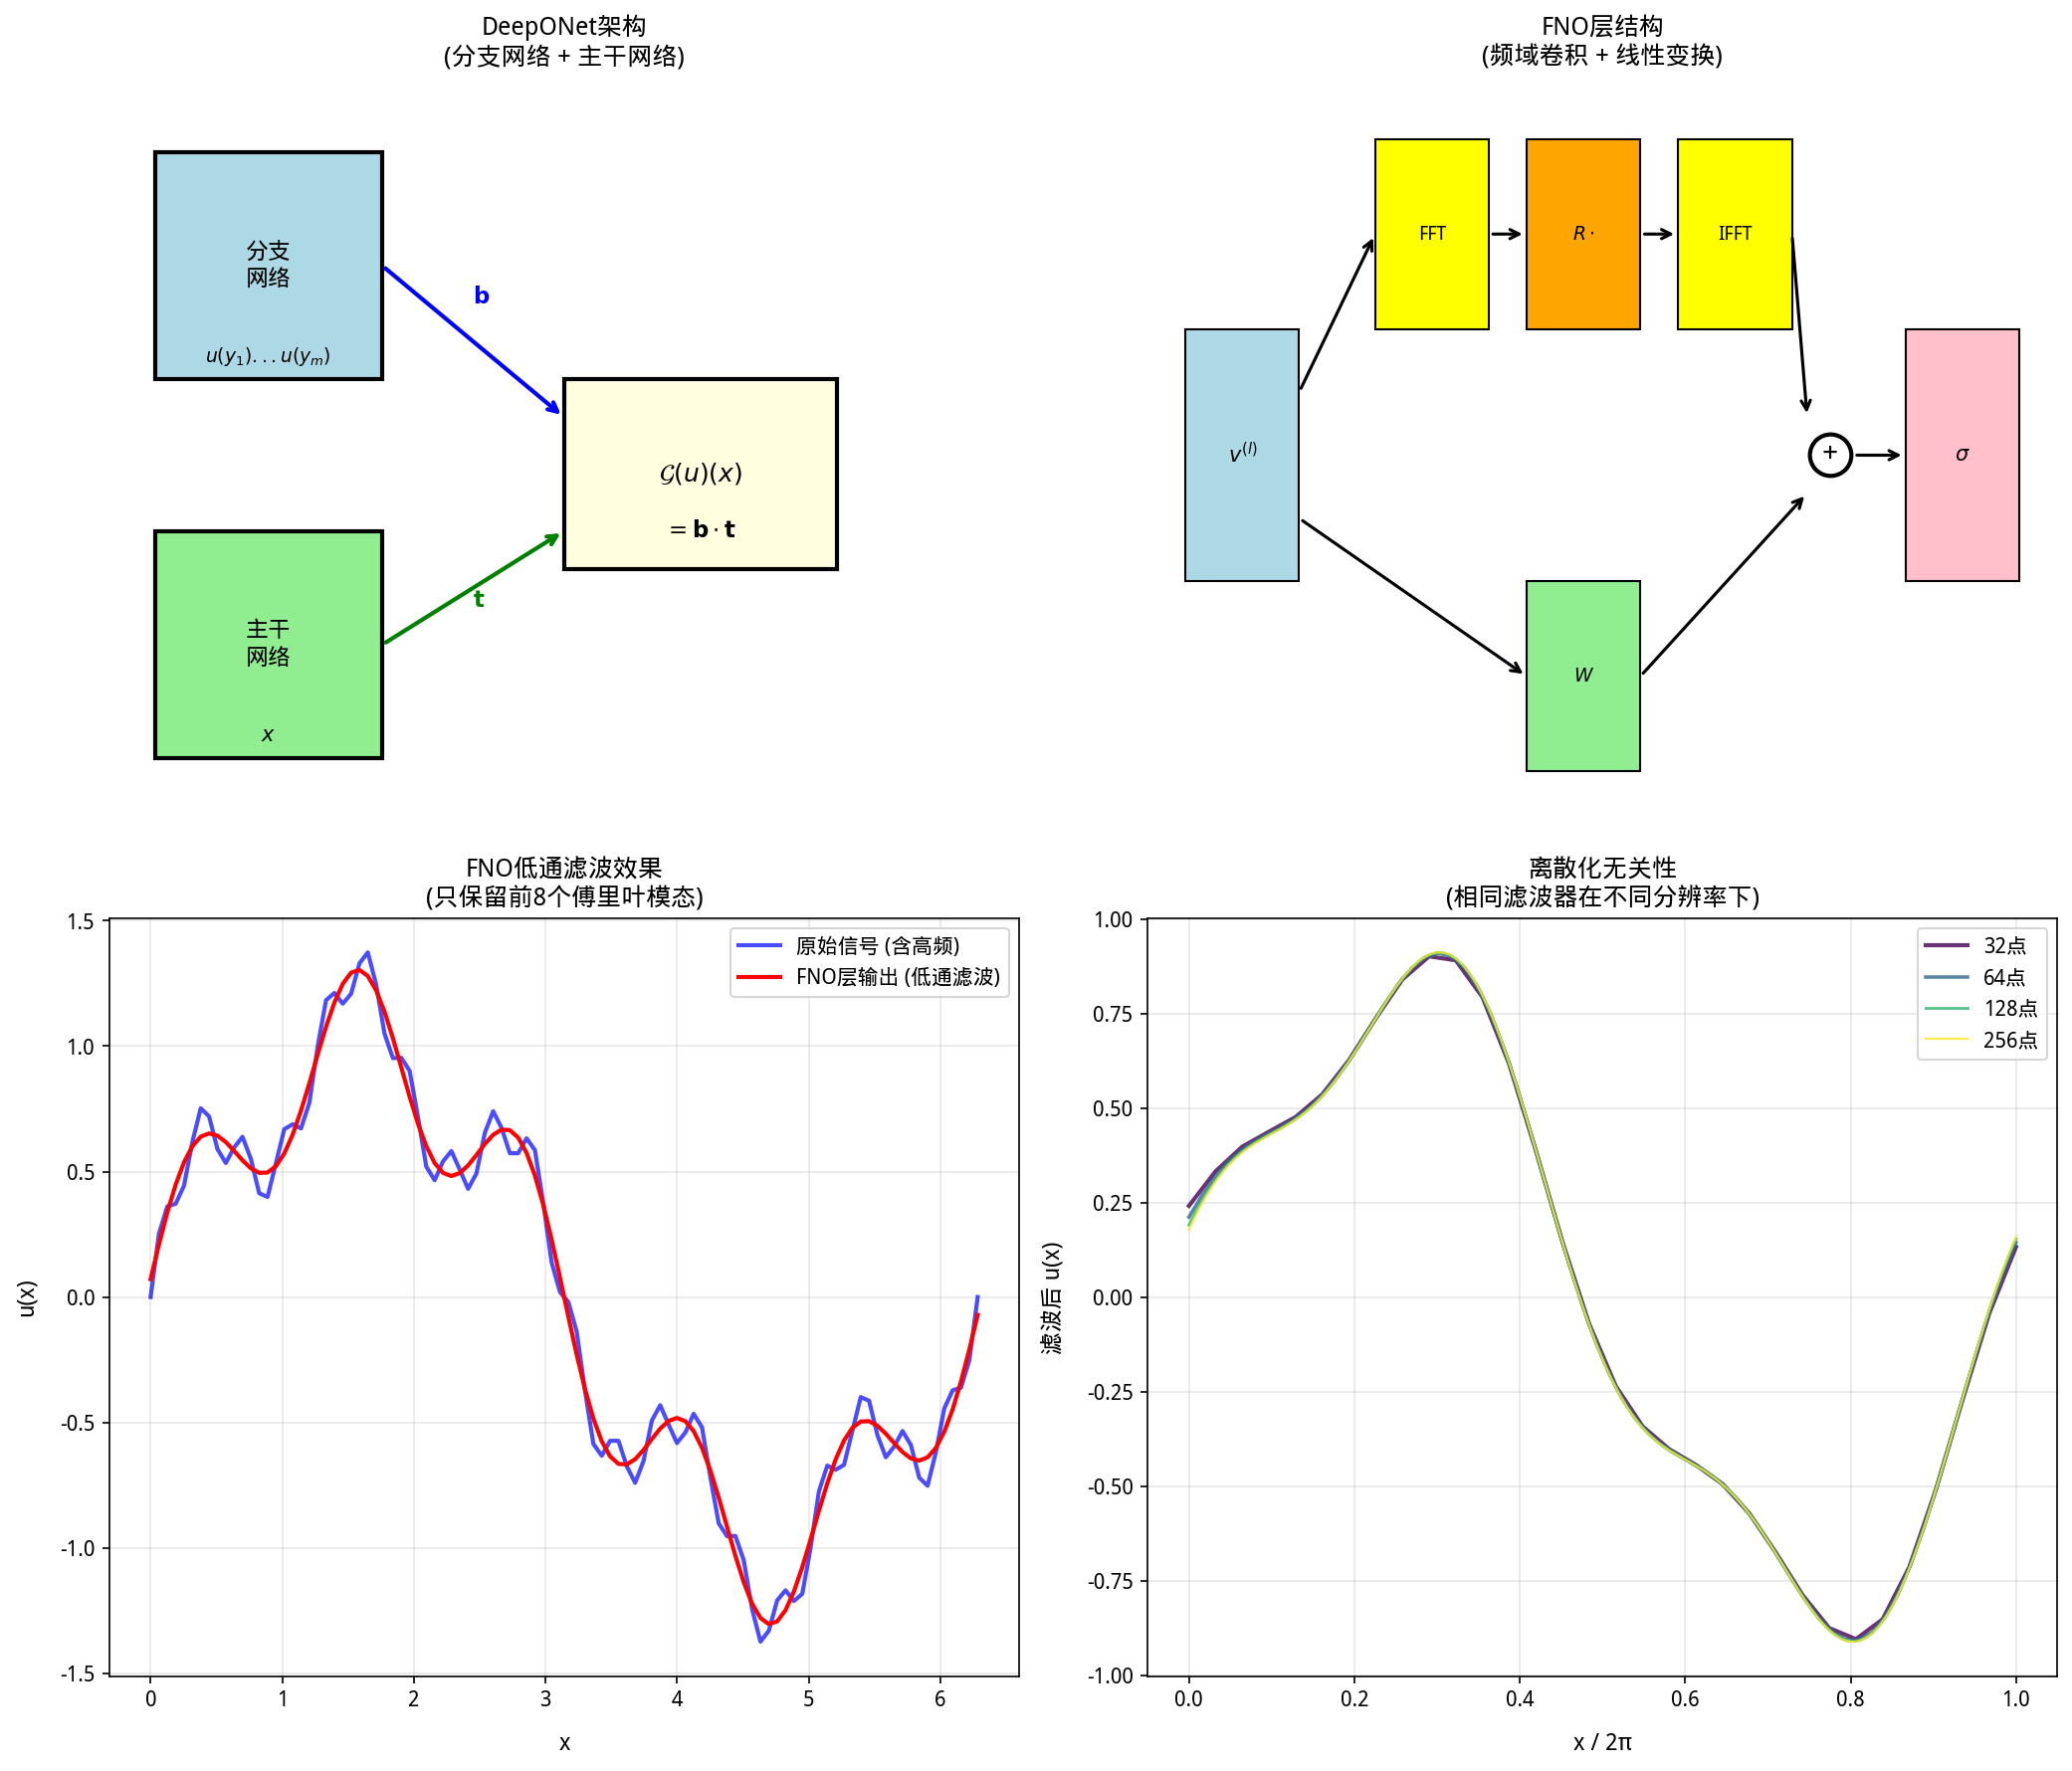
\includegraphics[width=0.95\textwidth]{figs_chap14/chap14_fig1.png}
\caption{神经算子概念演示。（1）DeepONet架构：分支网络处理输入函数采样值，主干网络处理查询位置，输出通过内积合成——这是万能逼近定理的实现；（2）FNO频域滤波：在傅里叶空间对高频和低频分量进行不同处理，体现频域操作的离散化无关性；（3）离散化无关性验证：同一个算子在不同分辨率网格上的输出保持一致性，实现零样本超分辨率的关键特性。}
\label{fig:chap14_neural_operator}
\end{figure}

% ====================================================================================
\section{本章小结}
% ====================================================================================

\begin{enumerate}
    \item \textbf{从函数到算子}：PINN 学一个特定问题的解 $u(x)$；神经算子学"条件函数 $\to$ 解函数"的映射 $\mathcal{G}$，一次训练、任意条件。
    \item \textbf{离散化无关性}：模型逼近的是连续算子，训练分辨率和推理分辨率可以不同（零样本超分辨率）。
    \item \textbf{数学统一}：所有神经算子都可以写成积分算子 $v(x) = \int \kappa(x, y) u(y)\,dy$，不同架构只是参数化积分核 $\kappa$ 的不同方式；线性情形下这个核就是格林函数，也就是第6章 $K^{-1}$ 的连续版本。
    \item \textbf{两种主流架构}：DeepONet（基函数展开：分支网络给系数、主干网络给基函数，理论清晰、通用）与 FNO（频域卷积：效率高、分辨率无关，适合周期 / 光滑问题）。
    \item \textbf{与 PINN 的关系}：PINN 把物理约束写进损失、针对单个问题；神经算子把物理隐含在数据里、针对一类问题；PINO 把两者结合。
\end{enumerate}

\begin{physicalmeaning}
\textbf{$\lambda$ 在本章的意义}：第1章的 $\lambda$ 回答"这条约束放松一点，目标变多少"；PDE 是一整族约束——每个点 $\xi$ 处方程都要成立——于是影子价格也成了一个函数：在 $\xi$ 处加一个单位源，解在 $x$ 处变化 $G(x, \xi)$。格林函数就是 PDE 约束的影子价格表，第9章的伴随变量就是这张表乘上目标的梯度。神经算子学的就是这张表。代价也在这里：纯数据驱动的 DeepONet / FNO 没有显式约束，$\lambda \equiv 0$，没有人替物理定律"看门"——这就是"应用案例"一节警告"预测可能违反守恒律"的根源；PINO 把第13章的乘子请回来，正是为了补上这个缺口。
\end{physicalmeaning}

% ====================================================================================
\section{习题}
% ====================================================================================

\paragraph{计算题}
\begin{enumerate}
    \item \textbf{格林函数与DeepONet}：
    考虑一维泊松方程$-u''(x) = f(x)$，$u(0) = u(1) = 0$。
    
    \begin{enumerate}
        \item 写出格林函数$G(x, y)$的表达式
        \item 如果用DeepONet学习从$f$到$u$的映射，分支网络的输入是什么？主干网络的输入是什么？
        \item DeepONet学到的$\sum_k b_k(f) t_k(x)$与格林函数表示$\int G(x,y) f(y) dy$有什么联系？
    \end{enumerate}
    
\end{enumerate}

\paragraph{编程题}
\begin{enumerate}
    \setcounter{enumi}{1}
    \item \textbf{实现2D FNO}：
    将本章的1D FNO代码扩展到2D情况：
    \begin{enumerate}
        \item 实现\code{SpectralConv2d}类
        \item 实现\code{FNO2d}类
        \item 在Darcy流问题上测试：给定渗透率场$a(x,y)$，预测压力场$u(x,y)$
    \end{enumerate}
    
    \textbf{提示}：2D FFT使用\code{torch.fft.rfft2}和\code{torch.fft.irfft2}。
    
    \item \textbf{DeepONet变体}：
    实现以下DeepONet的变体，并比较它们的性能：
    \begin{enumerate}
        \item \textbf{PI-DeepONet}：在损失函数中加入物理约束
        \item \textbf{Multi-output DeepONet}：主干网络输出多个查询点的结果
        \item \textbf{Deep DeepONet}：在内积之后再加一个MLP
    \end{enumerate}
    
\end{enumerate}

\paragraph{思考题}
\begin{enumerate}
    \setcounter{enumi}{3}
    \item \textbf{理解离散化无关性}：
    解释为什么以下操作不具有离散化无关性：
    \begin{enumerate}
        \item 全连接层 $y = Wx + b$，其中$x \in \mathbb{R}^n$
        \item 固定大小的卷积核
    \end{enumerate}
    
    提出一种使它们具有离散化无关性的修改方案。
    
    \item \textbf{神经算子的局限}：
    讨论神经算子在以下场景中可能遇到的困难：
    \begin{enumerate}
        \item 激波问题（Burgers方程在黏性趋近于零时）
        \item 湍流（高雷诺数Navier-Stokes方程）
        \item 多尺度问题（例如大气-海洋耦合）
    \end{enumerate}
    
    你能想到什么改进方法？
    
    \item \textbf{算子学习 vs 传统数值方法}：
    比较神经算子和传统数值方法（如有限元）的优缺点。在什么情况下应该选择神经算子？在什么情况下应该坚持传统方法？
    
\end{enumerate}
